\documentclass[12pt]{article} % use larger type; default would be 10pt

\usepackage[utf8]{inputenc} % set input encoding (not needed with XeLaTeX)
\usepackage{geometry} % to change the page dimensions
 \geometry{margin=1in} 
\usepackage{graphicx} % support the \includegraphics command and options

\begin{document}

\section*{Figures}

Figure 1: Results of path analyses in commodity and seed fields. \emph{Field Edge Distance} refers to the distance to the edge of the field (and location of HB apiary) and \emph{Shelter Distance} refers to the distance to the nearest LCB shelter. The width of each arrow is proportional to the effect size of each component path (number also displayed), with black and red lines representing positive and negative effects, respectively. Transparent arrows show path coefficients whose 95\% CIs overlapped zero.

\vspace{0.5cm}

Figure 2: Partial effect of distance from a) honey bee apiaries (at edge of the field), b) leafcutter shelters, and c) female bay position on visitation rates, with shaded regions and line ranges showing 95\% CIs. Commodity fields are shown at a stocking rate of 40 hives (black line), while stocking rates are at 160 hives in seed fields (yellow line).

\vspace{0.5cm}

Figure 3: Partial effect of a) visitation rate, b) distance from apiary (HB) or shelter (LCB), and c) female bay position on pollen deposition, with shaded regions and line ranges showing 95\% CIs.

\vspace{0.5cm}

Figure 4: Partial effect of pollen deposition (top row) and plant size (bottom row) on flower survival, seeds per pod, and seed size, with shaded regions showing 95\% CIs.

\vspace{0.5cm}

Figure 5: Simulated effect of honey bee distance and leafcutter distance on seed size (mg/seed, first column) and total yield (tonnes/hectare, second column), using coefficients from paths for simulation. Shaded areas shown in a \& b are 95\% quantiles for the simulations. Lines on panels c - f are isolines of constant seed size (c, e) or yield (d, f).

\clearpage

\begin{figure}
    \centering
    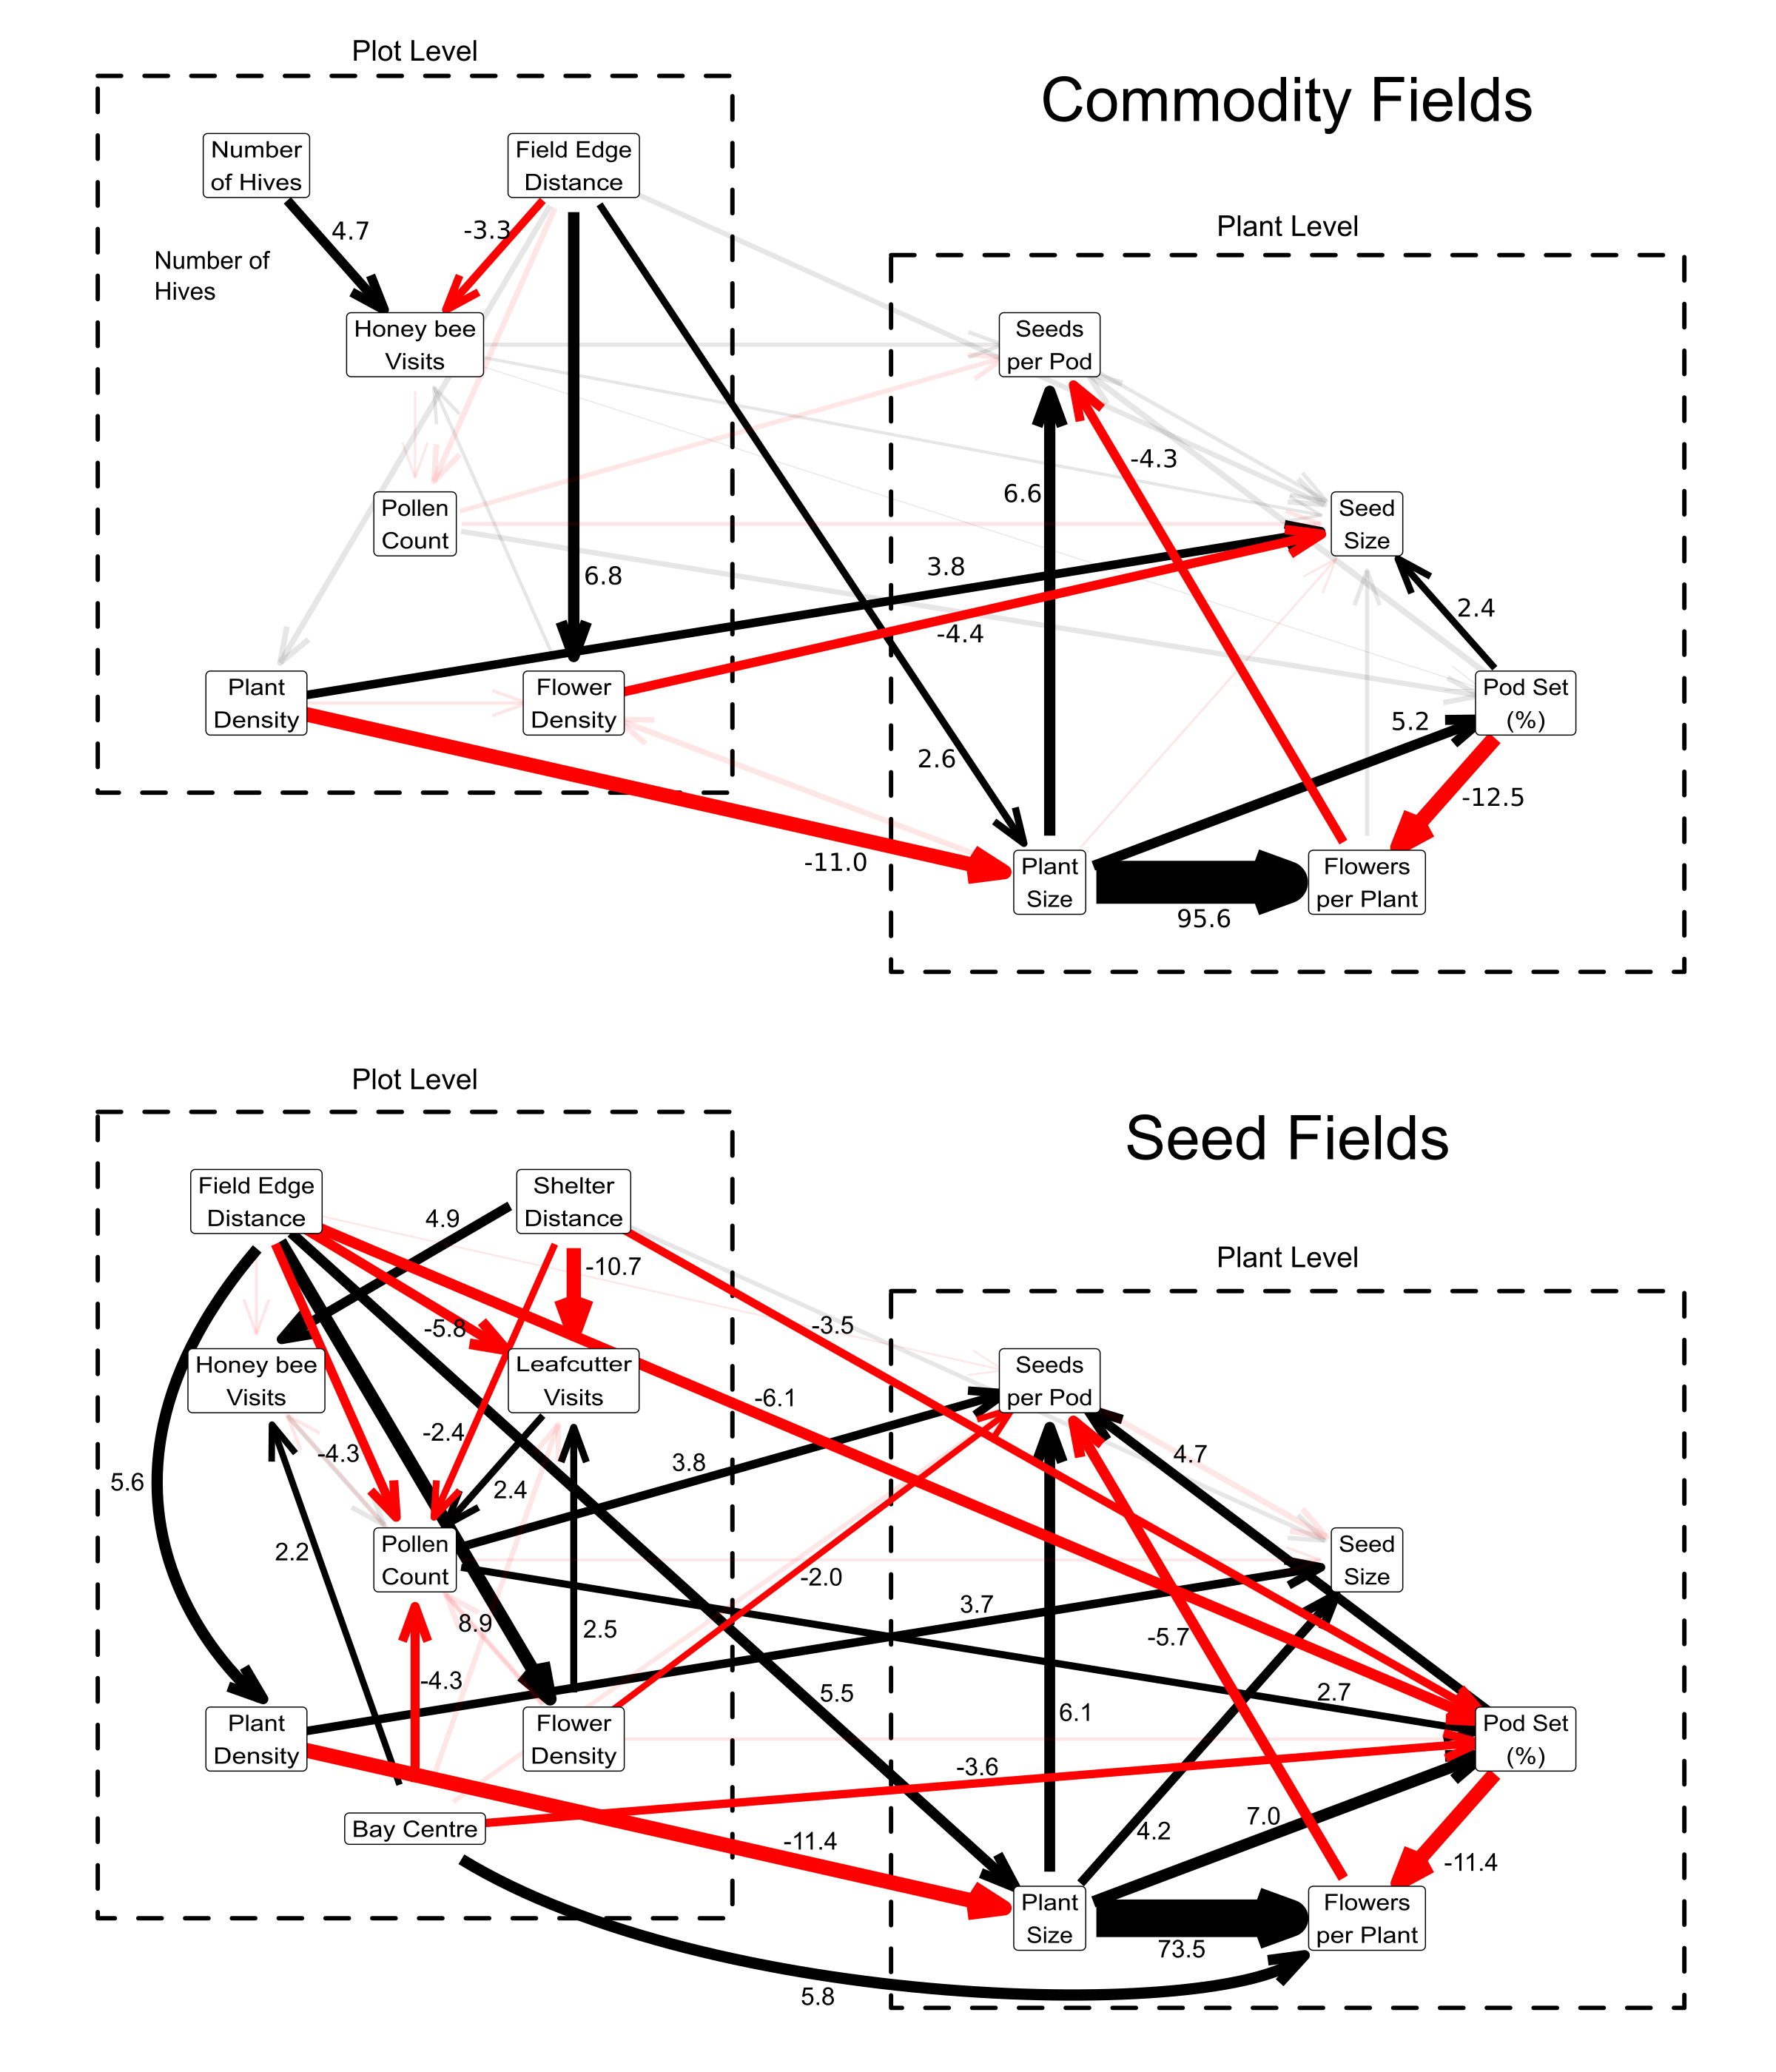
\includegraphics[width=\textwidth,keepaspectratio=true]{allSEM.png}
\end{figure}

\begin{figure}
    \centering
    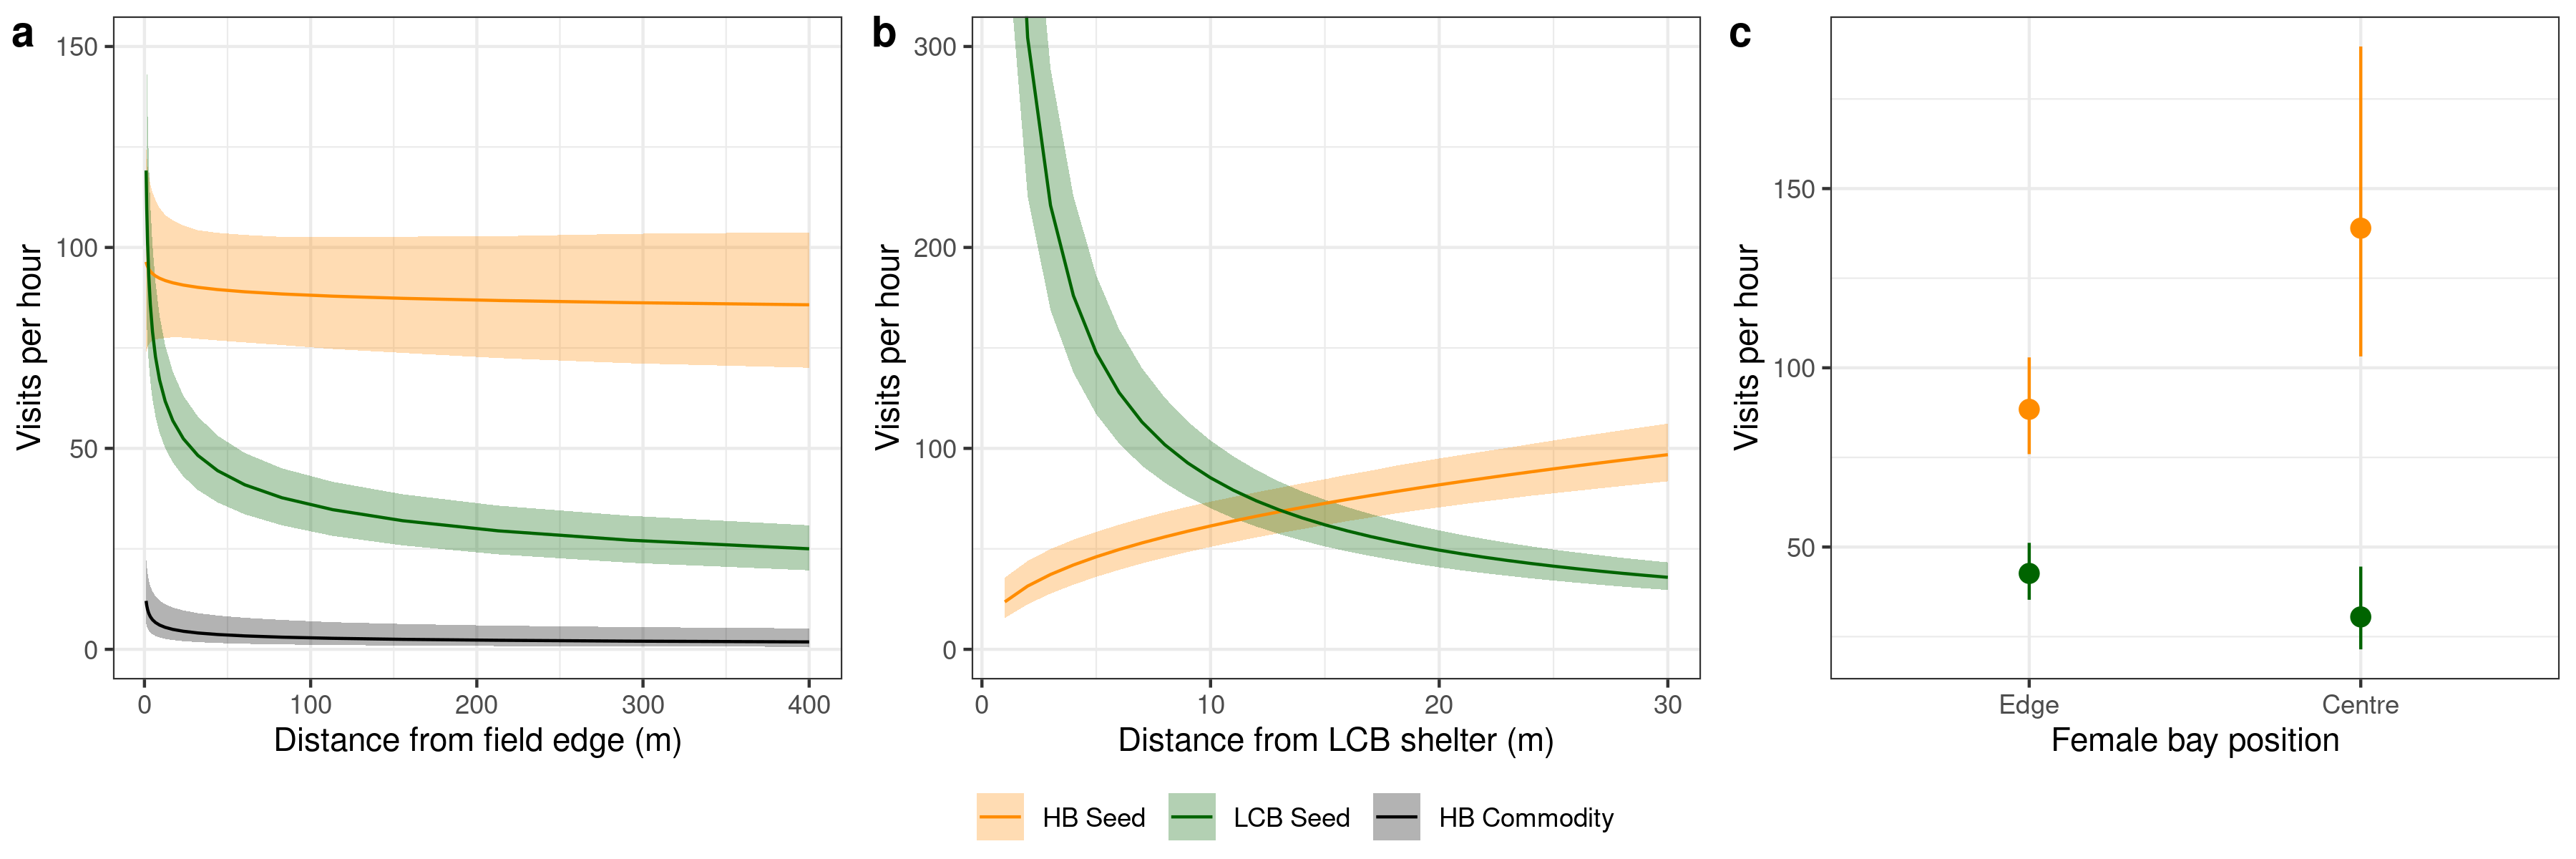
\includegraphics[width=\textwidth,keepaspectratio=true]{allVisits.png}
\end{figure}

\begin{figure}
    \centering
    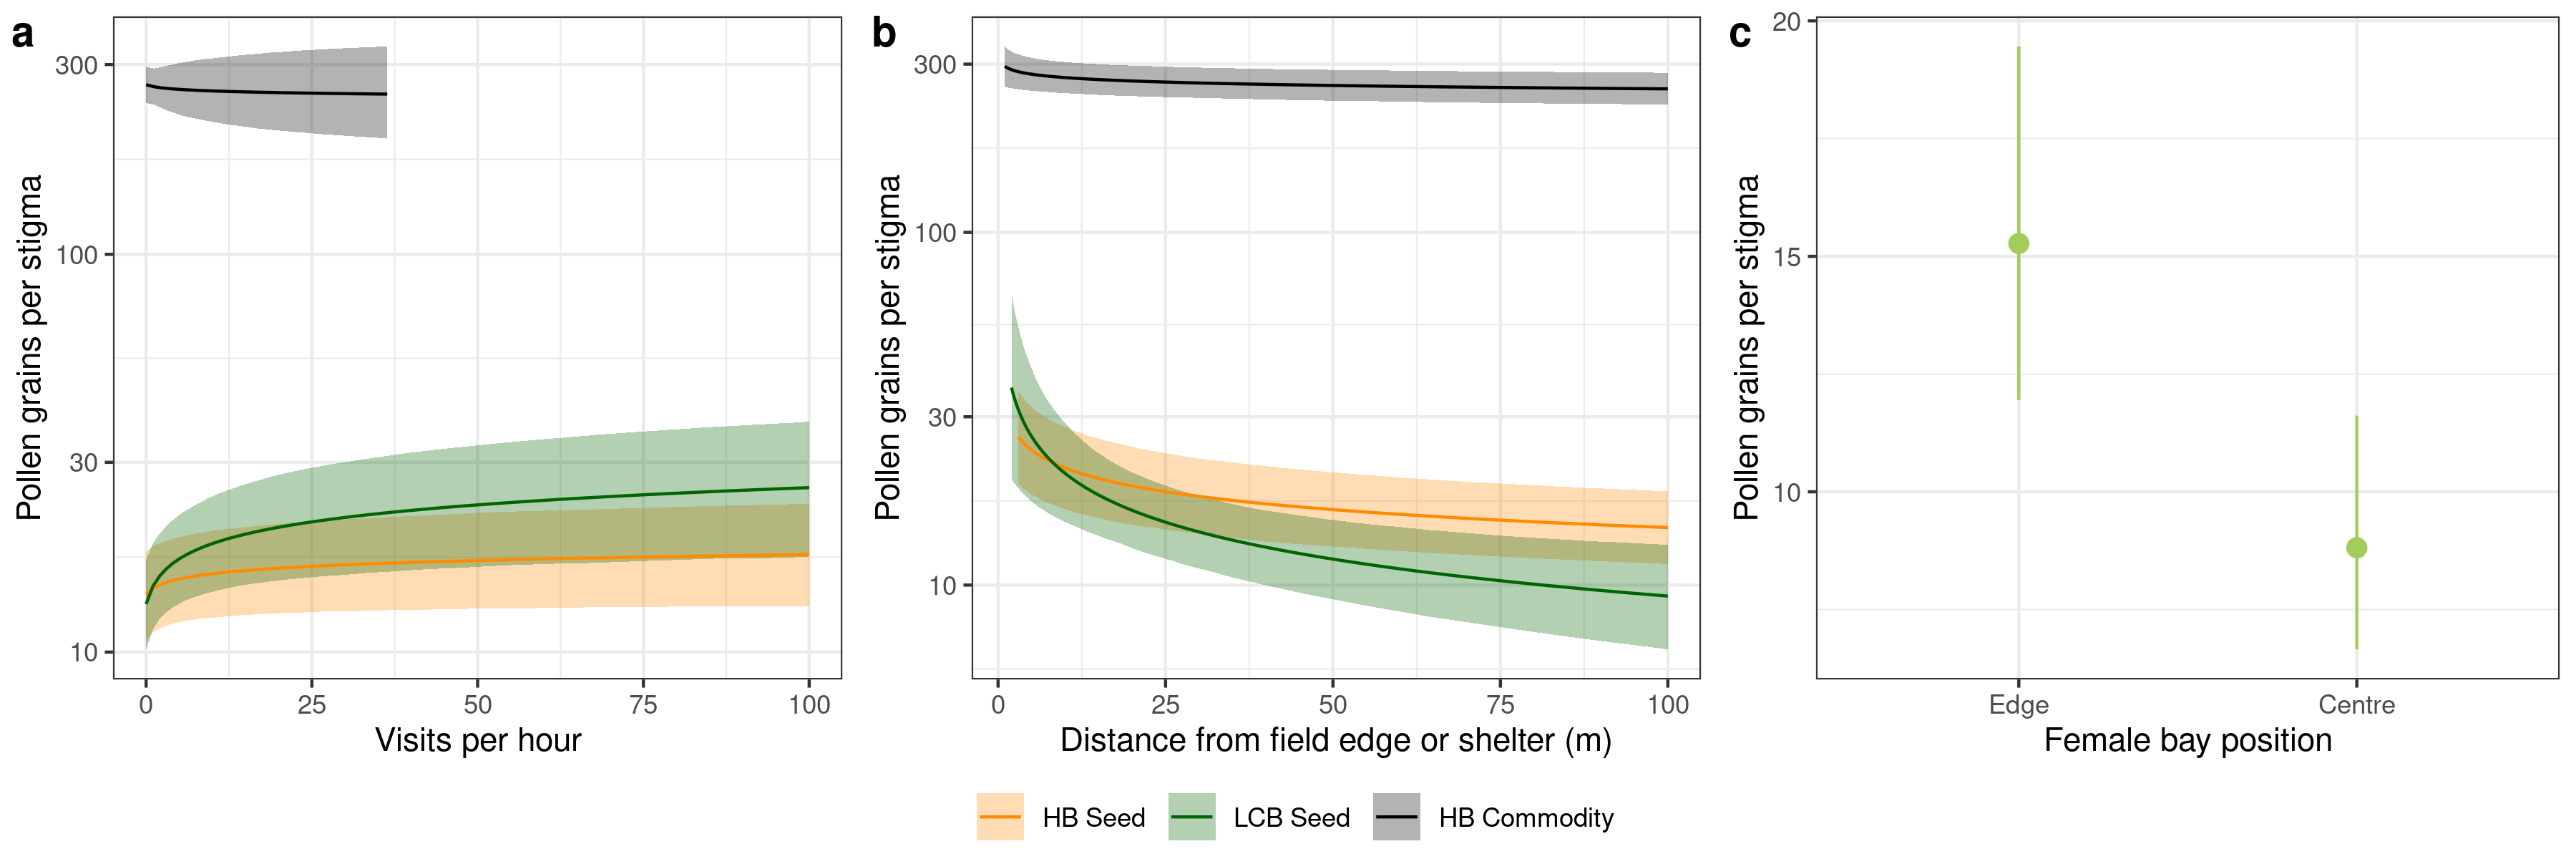
\includegraphics[width=\textwidth,keepaspectratio=true]{allPollen.png}
\end{figure}

\begin{figure}
    \centering
    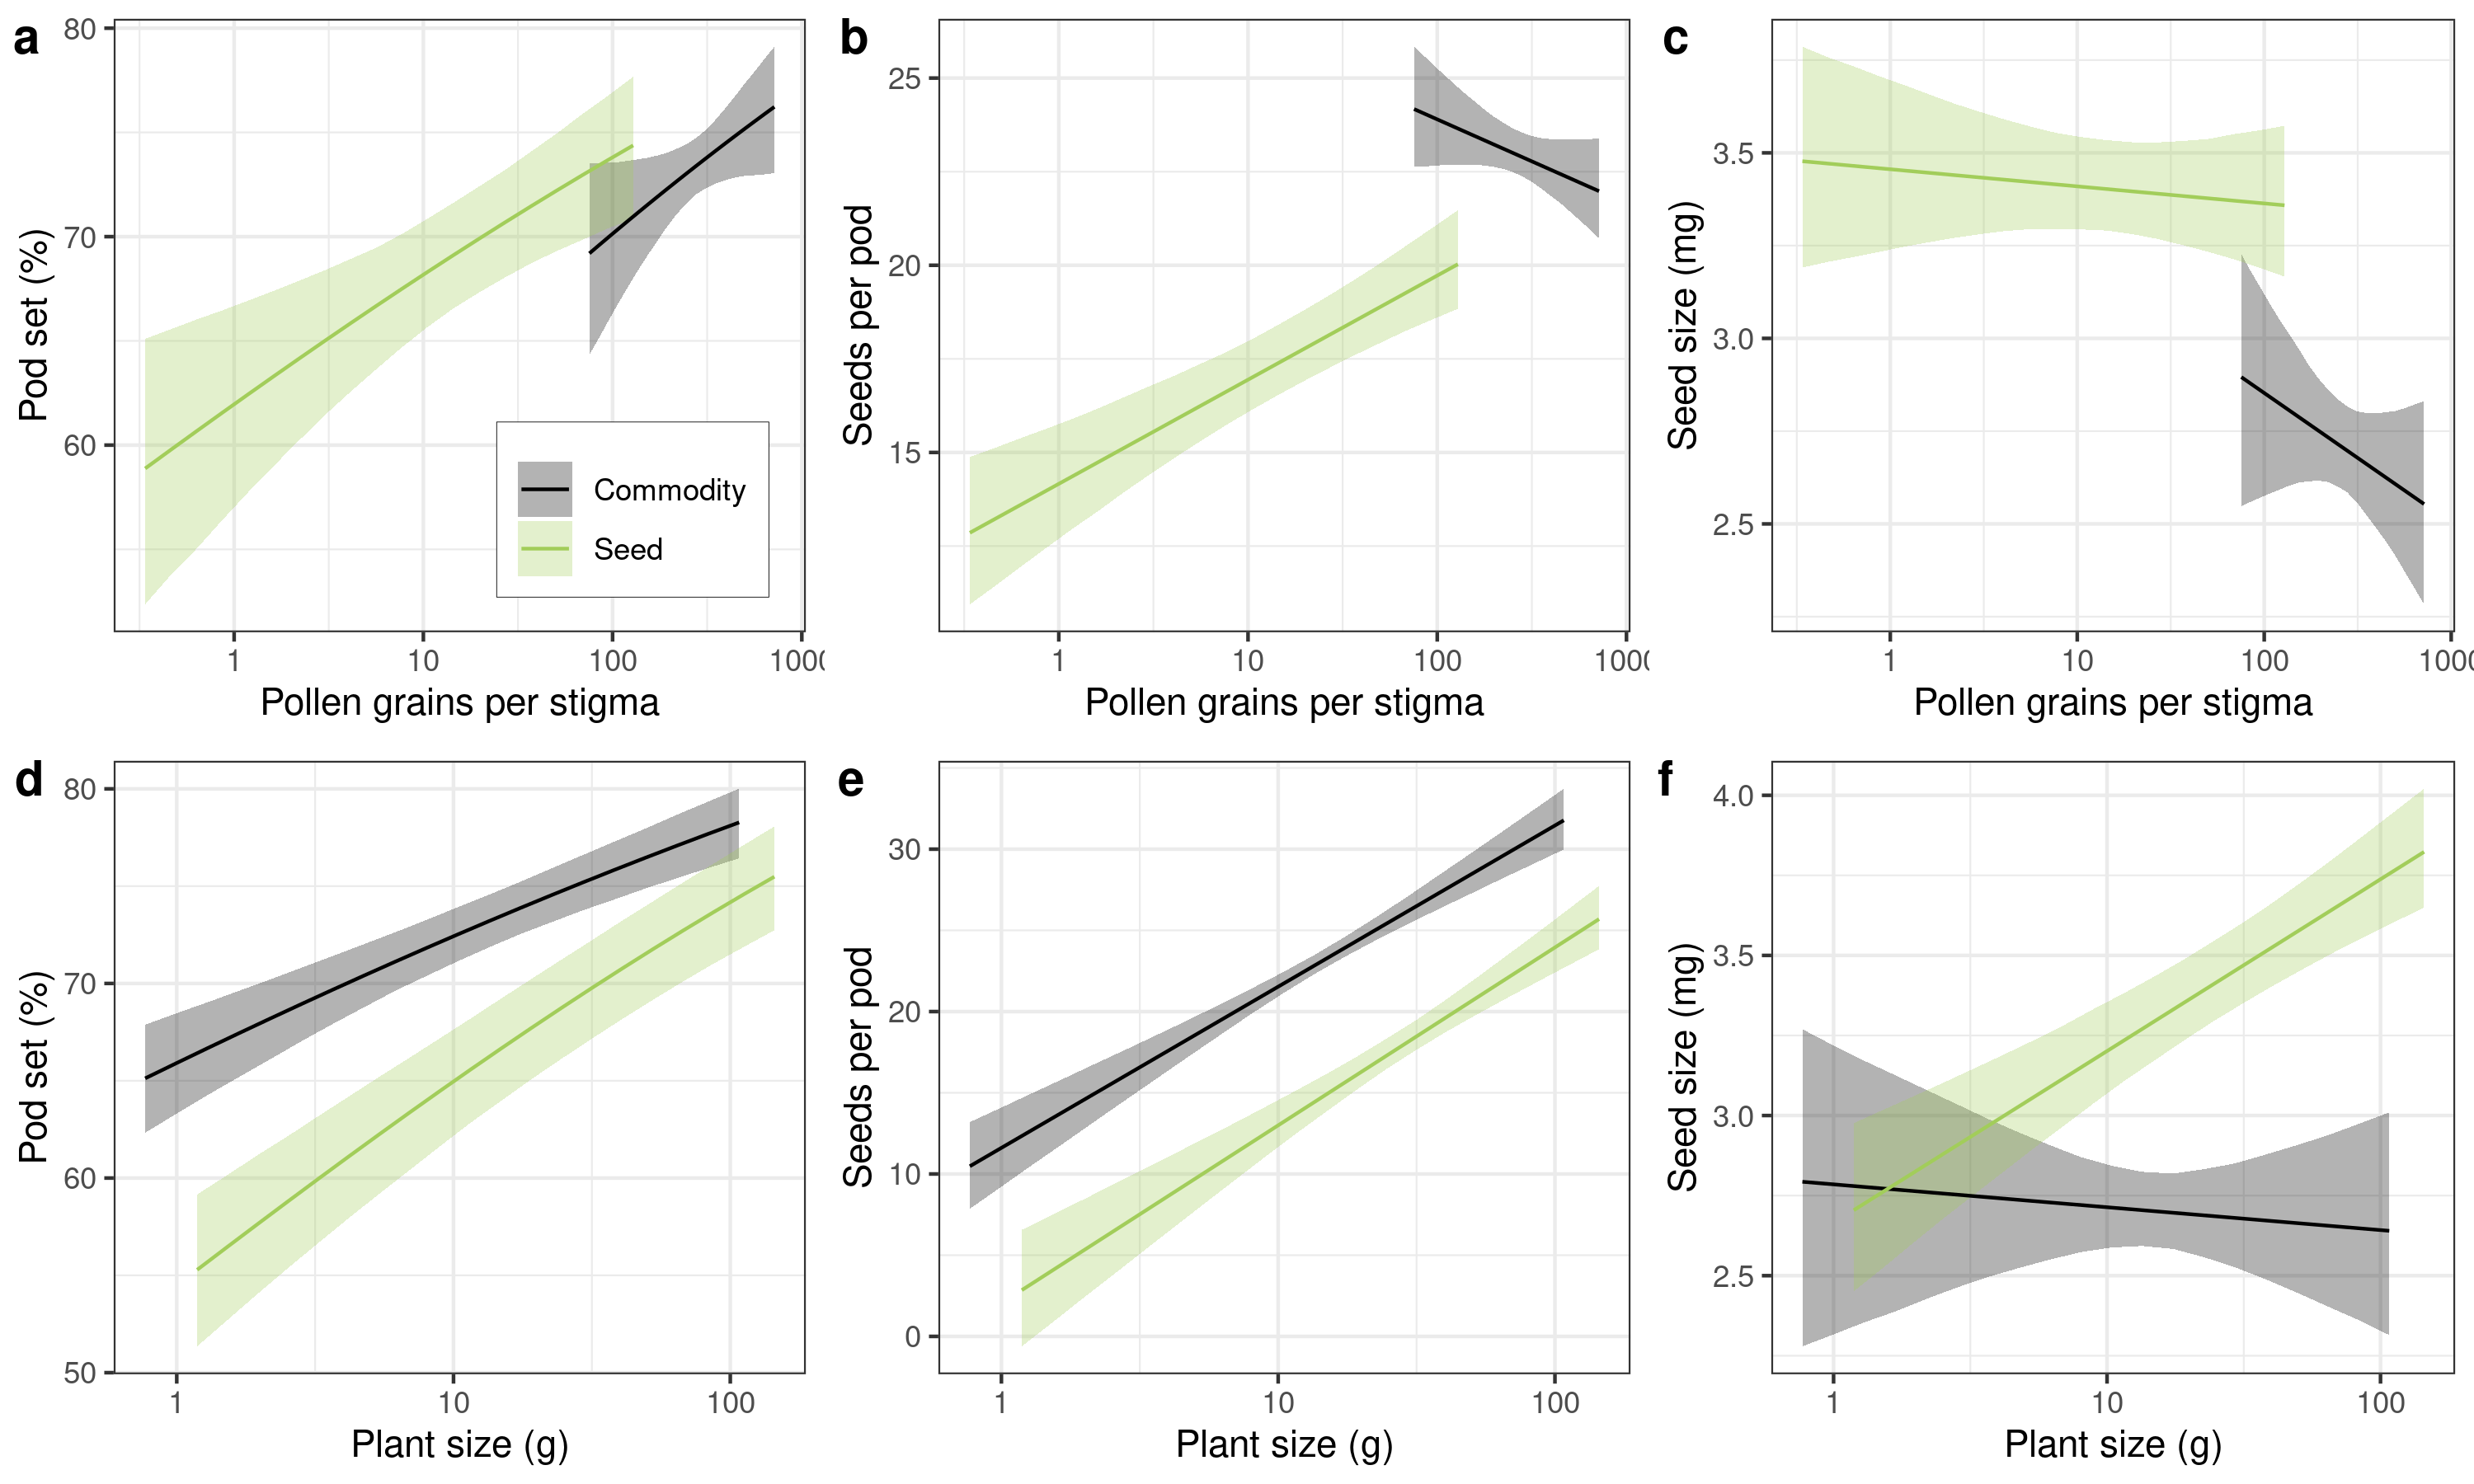
\includegraphics[width=\textwidth,keepaspectratio=true]{allSeeds.png}
\end{figure}

\begin{figure}
    \centering
    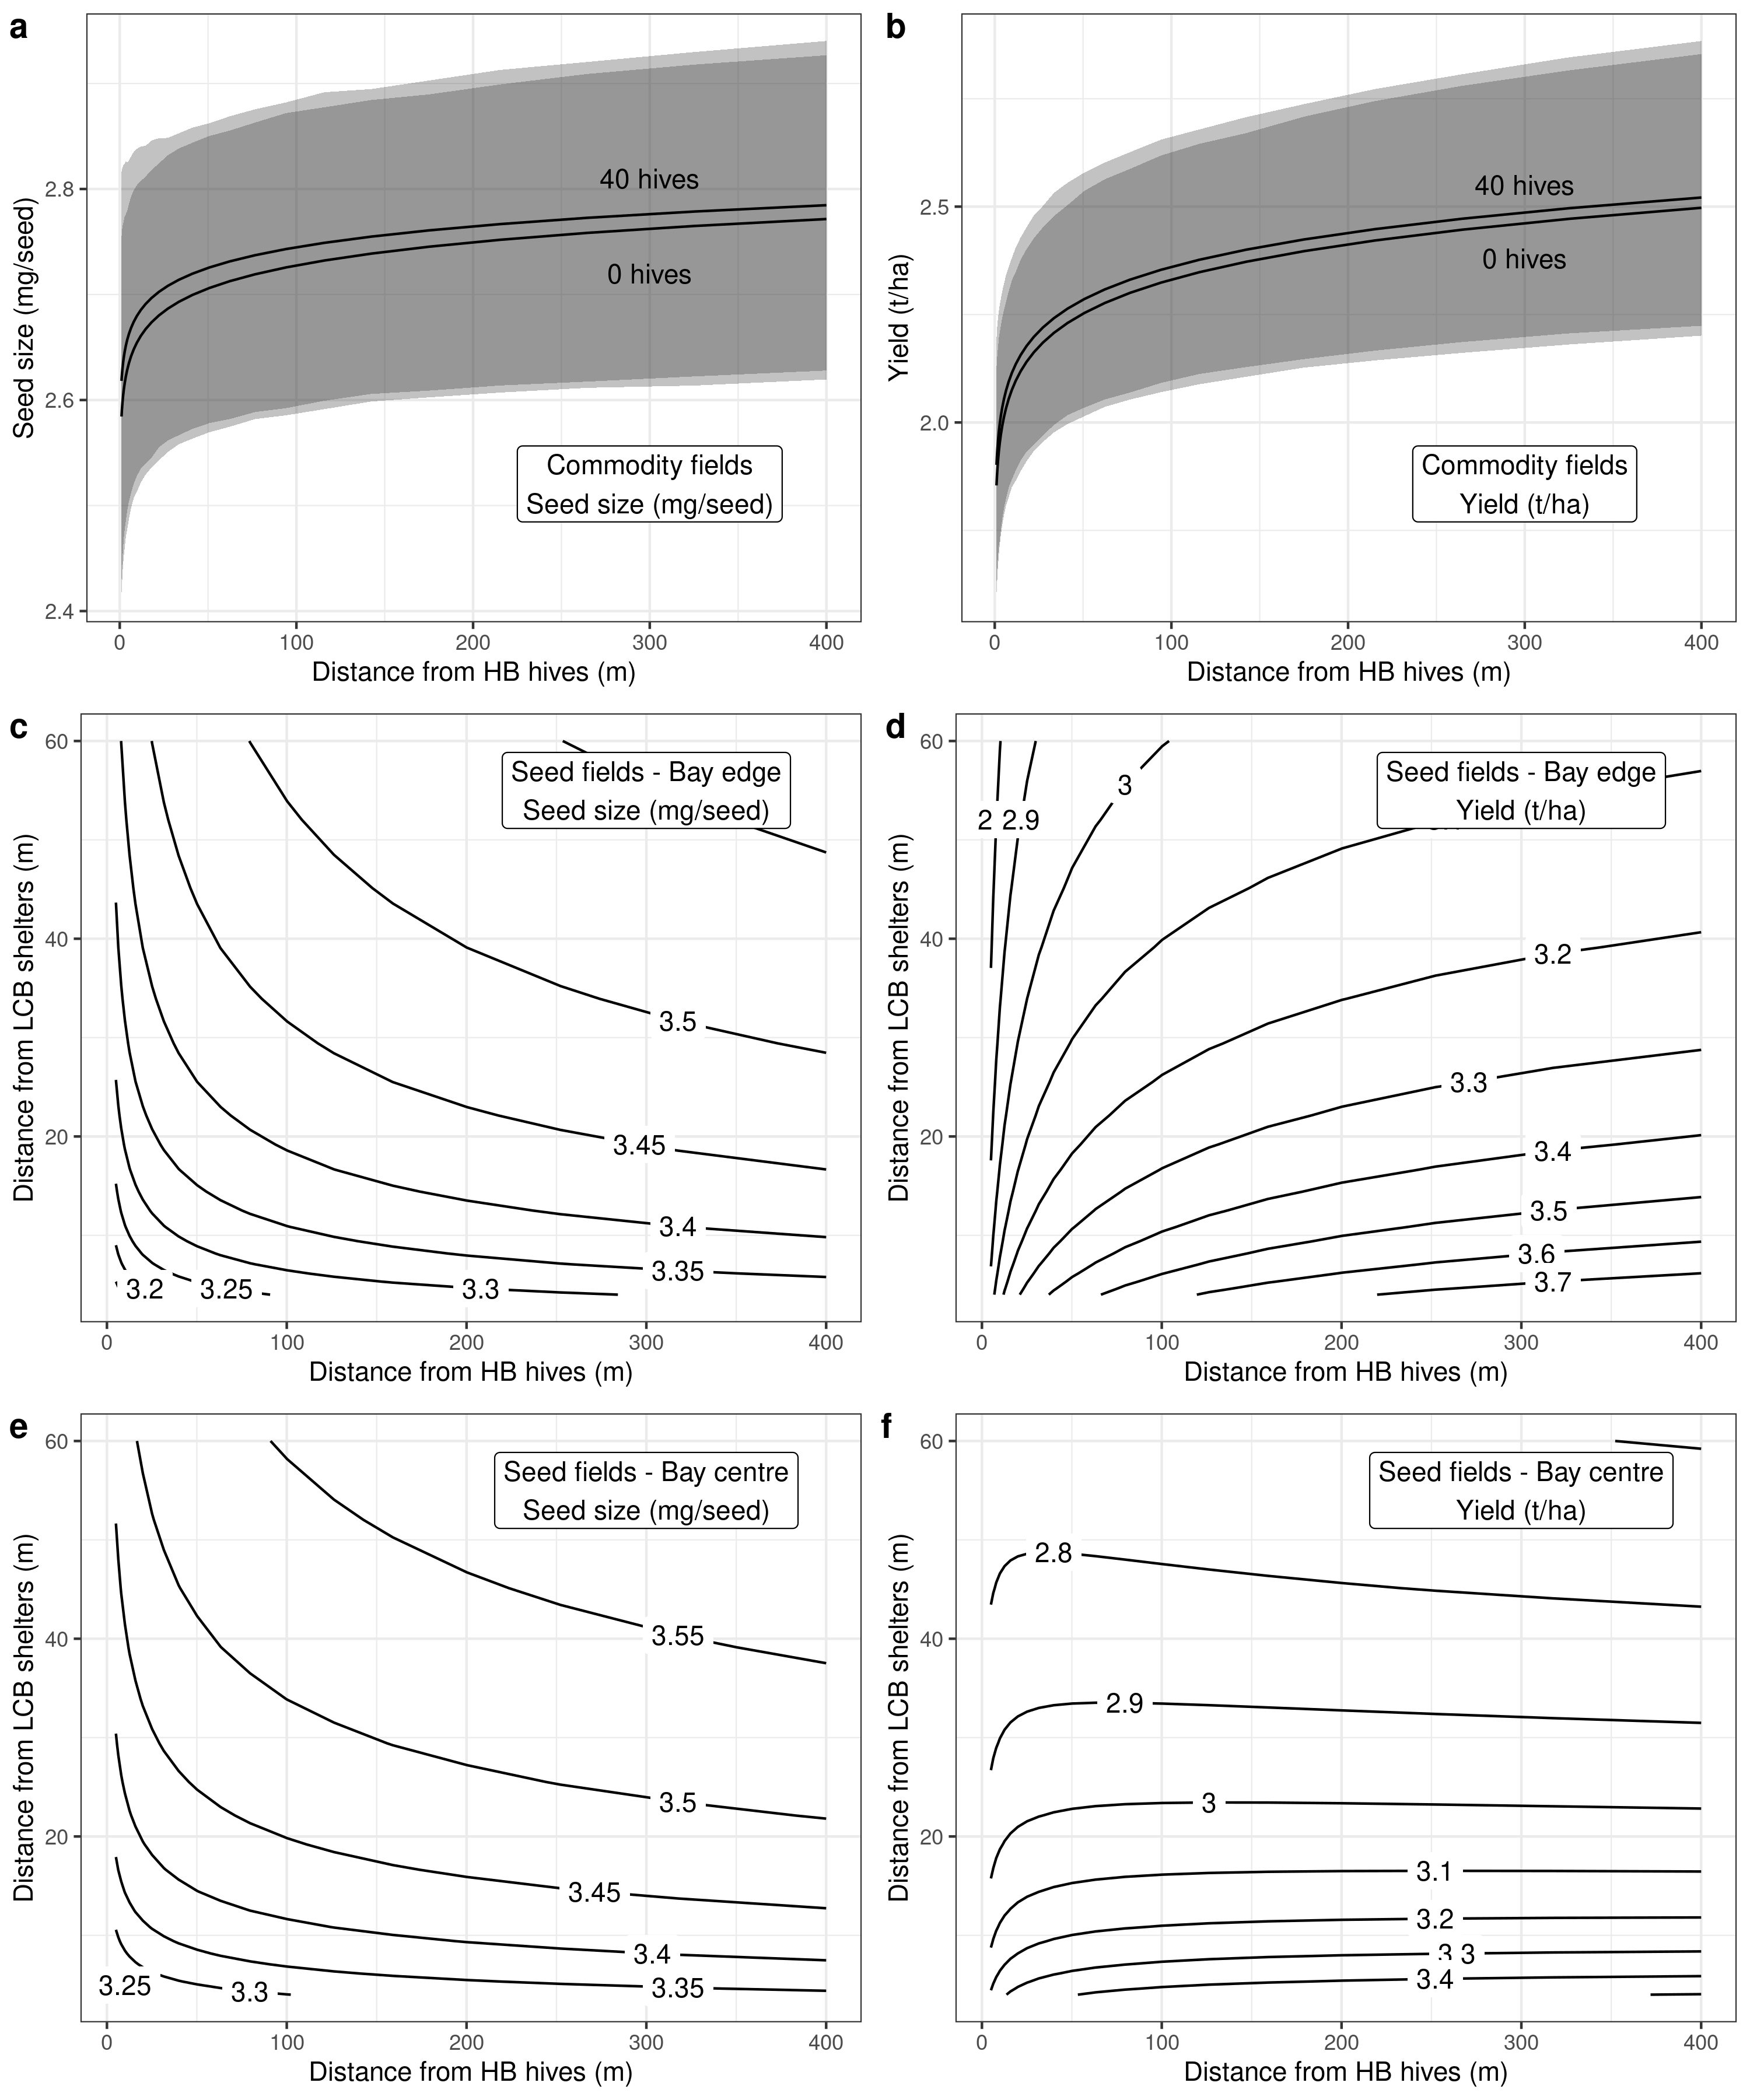
\includegraphics[width=\textwidth,keepaspectratio=true]{allYield.png}
    \label{fig:allYield}
\end{figure}

\end{document}